%%%%%%%%%%%%%%%%%%%%%%%%% 
%% SITE A GARDER : http://titilog.free.fr/


\documentclass[10pt]{beamer}
% \includeonlyframes{yy}
\usepackage[french]{babel}
\usepackage{color, colortbl}
\definecolor{Gray}{gray}{0.9}
\newcolumntype{g}{>{\columncolor{Gray}}c}
\hypersetup{%
  % pdfborder = {0 0 0},
  colorlinks, urlcolor=blue, linkcolor=, }

\makeatletter \let\@mycite\@cite
\def\@cite#1#2{{\hypersetup{linkcolor=mLightBlue}[{#1\if@tempswa ,
      #2\fi}]}} \makeatother

\usetheme{m} %%%%%
% \usepackage[version=3]{mhchem}
\usepackage{caption}
\captionsetup[figure]{labelformat=empty}
\usepackage{fontspec}
\usepackage{xcolor}
\usepackage{siunitx}
% \usepackage[backend=bibtex]{biblatex} \usepackage[square]{natbib}
% \bibliography{main}
\usepackage[]{algorithm2e}
\usefonttheme[onlymath]{serif} \usepackage{amsmath}
\usepackage{subcaption} \usepackage{appendixnumberbeamer}
\usepackage{tabularx, booktabs} \usepackage{multirow}
\usepackage{multicol} \usepackage{array} \usepackage{pbox}
\usepackage{mathtools}
\usepackage{adjustbox}
\definecolor{darkred}{HTML}{D38989}
\definecolor{darkgreen}{HTML}{66D191}
\PassOptionsToPackage{enumerate}{shortlabels} \newcommand\ExtraSep
{\dimexpr\cmidrulewidth\relax}
\captionsetup{font=scriptsize,labelfont=scriptsize}
% \addtobeamertemplate{background canvas}{\transfade[duration=0.05]}{}


\title{Fusion d'images IRM et MALDI en 3D}
\subtitle{Dernières avancées}

\author{{Florent \textsc{Grélard}\\
    David \textsc{Legland}, Mathieu \textsc{Fanuel}, Loïc \textsc{Foucat}, Hélène \textsc{Rogniaux}}} \titlegraphic{\hspace*{0.18\textwidth}~%
  
\includegraphics[width=0.26\textwidth]{fig/logo-inrae}\hspace*{0.18\textwidth}~%
  
\includegraphics[width=0.26\textwidth]{fig/logo-bibs.png}\hspace*{0.1\textwidth}~%
} \setbeamercolor{bbb}{fg=red}

\let\oldfootnotesize\footnotesize
\renewcommand*{\footnotesize}{\oldfootnotesize\tiny}
\newcommand\labelitemi{$\bullet$}
\renewcommand{\thefootnote}{[\arabic{footnote}]}
% \newrobustcmd*{\footlessfullcite}{\AtNextCite{\renewbibmacro{in:}{}\renewbibmacro{year:}{}}\footfullcite}
% \newrobustcmd*{\lessfullcite}{\AtNextCite{\renewbibmacro{in:}{}\renewbibmacro{year:}{}}\fullcite}

\newcommand{\cfbox}[2]{%
    \colorlet{currentcolor}{.}%
    {\color{#1}%
    \fbox{\color{currentcolor}#2}}%
}


\newcommand{\backupbegin}{ \newcounter{framenumberappendix}
  \setcounter{framenumberappendix}{\value{framenumber}} }
\newcommand{\backupend}{
  \addtocounter{framenumberappendix}{-\value{framenumber}}
  \addtocounter{framenumber}{\value{framenumberappendix}} }
% http://mcclinews.free.fr/latex/introbeamer/les_couleurs.html
\begin{document}

% affiche le logo en bas à droite
% \logo{
\includegraphics[height=0.5cm]{fig/logo-inra}}
% enlève la barre de navigation
\setbeamertemplate{navigation symbols}{ }
\setbeamertemplate{blocks}[rounded][shadow=false]
% Ombre aux blocks
\setbeamertemplate{caption}{\insertcaption}

\date{15 octobre 2020} % set the Date
% \AtBeginSection[]{
%	\begin{frame}[plain]{Sommaire}
%   \tableofcontents[currentsection, hideothersubsections]
%	\end{frame}
% } \renewcommand{\insertnavigation}[1]{}

% \AtBeginSection[]{

% }

% \institute{INRAE de Nantes}
\makeatletter
\AtBeginPart{%
  \beamer@tocsectionnumber=0\relax
  \setcounter{section}{0}
}
\makeatother

\begin{frame}[plain]
  \titlepage
\end{frame}


\section{Chaîne de traitement}

\begin{frame}{Chaîne de traitement 3D}


  \begin{enumerate}
  \item<2-> IRM: ajustement de \textbf{fonctions exponentielles}
  \item<3-> MALDI: \textbf{normalisation} des images
  \item<4-> Détermination des \textbf{correspondances} et \textbf{recalage 3D}
  \item<5-> \textbf{Visualisation} d'images MS en 3D
  \end{enumerate}

  \begin{figure}[ht]
    \centering
    \includegraphics<1>[width=0.8\textwidth]{fig/workflow3D_0}%
    \includegraphics<2>[width=0.8\textwidth]{fig/workflow3D_1}%
    \includegraphics<3>[width=0.8\textwidth]{fig/workflow3D_2}%
    \includegraphics<4>[width=0.8\textwidth]{fig/workflow3D_3}%
    \includegraphics<5>[width=0.8\textwidth]{fig/workflow3D_4}%
  \end{figure}
\end{frame}



\begin{frame}{Ajustement de fonctions exponentielles}
  
  \textbf{Précédemment}: trop peu d'échos $\Rightarrow$ surajustement, décroissance incomplète

  \begin{figure}[ht]
    \centering
    \begin{subfigure}[t]{0.5\textwidth}
      \centering
      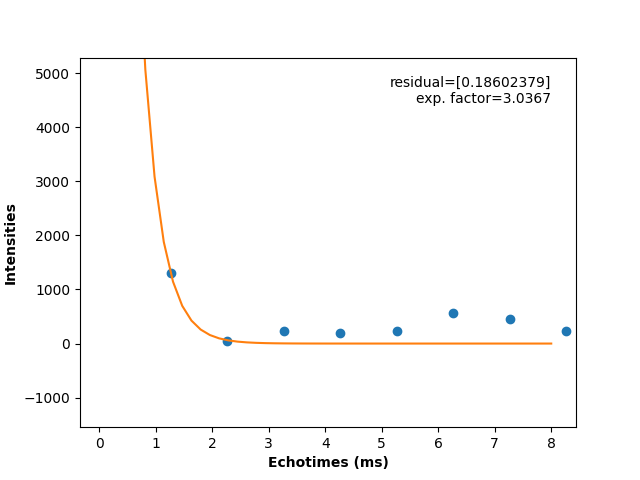
\includegraphics[width=0.8\textwidth]{fig/wrongfit_overfitting}
      \caption{Surajustement}
      \label{subfig:wrongfit_overfitting}
    \end{subfigure}%
    \begin{subfigure}[t]{0.5\textwidth}
      \centering
      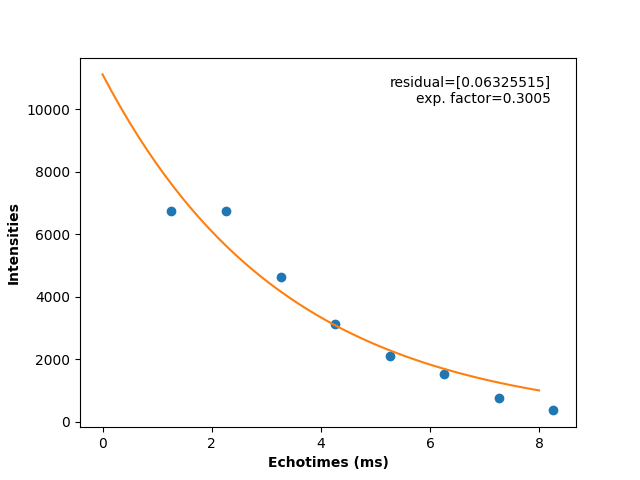
\includegraphics[width=0.8\textwidth]{fig/wrongfit_missing}
      \caption{Décroissance incomplète}
      \label{subfig:wrongfit_missing}
    \end{subfigure}%

  \end{figure}


  Nouvelles images: \textbf{plus d'échos} (8 $\rightarrow$ 16)

  \underline{Objectif :} modélisation \textbf{plus précise} de la décroissance du signal  
\end{frame}

\begin{frame}{Ajustement par morceaux}
  Modélisation par une \textbf{somme de fonctions exponentielles} (bi-exponentielle)

  Ajustement de \textbf{deux droites} sur le logarithme des intensités \textbf{par morceaux} :

  \begin{figure}[ht]
    \centering
    \begin{subfigure}[t]{0.5\textwidth}
      \centering
      \includegraphics<1-3>[width=0.95\textwidth]{fig/biexponential}%
      \includegraphics<4>[width=0.95\textwidth]{fig/biexponential_fitted}%
      \caption{Intensités}
      \label{subfig:}
    \end{subfigure}%
    \onslide<2->
    \begin{subfigure}[t]{0.5\textwidth}
      \centering
      \includegraphics<2>[width=0.95\textwidth]{fig/biexponential_log}%
      \includegraphics<3->[width=0.95\textwidth]{fig/biexponential_log_piecewise}
      \caption{Log des intensités}
      \label{subfig:}
    \end{subfigure}%
  \end{figure}

\end{frame}

\begin{frame}{Ajustement par morceaux}
  \textbf{Problème :} profils \textbf{mono-exponentiels} dans la cavité $\Rightarrow$ surajustements

  \begin{figure}[ht]
    \centering
    \begin{subfigure}[t]{0.5\textwidth}
      \centering
      \includegraphics<1>[width=0.9\textwidth]{fig/piecewise}%
      \includegraphics<2->[width=0.9\textwidth]{fig/piecewise_circled}
      \caption{Densité}
      \label{subfig:piecewise}
    \end{subfigure}%
    \onslide<3>
    \begin{subfigure}[t]{0.5\textwidth}
      \centering
      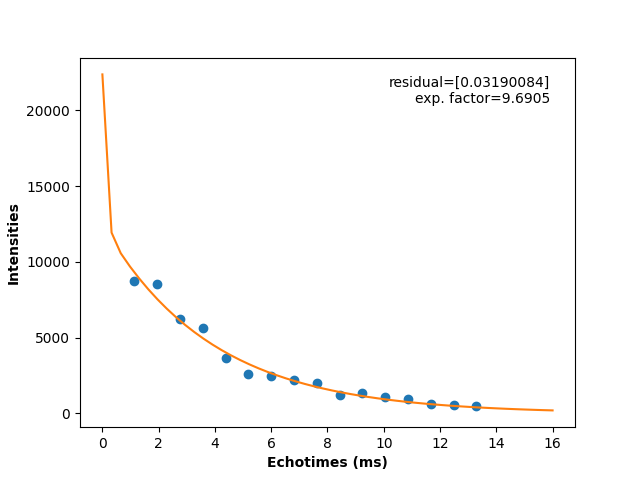
\includegraphics[width=0.9\textwidth]{fig/piecewise_defect}
      \caption{Surajustement}
      \label{subfig:piecewise_defect}
    \end{subfigure}%

  \end{figure}

\end{frame}

\begin{frame}{Ajustement de fonction mono-exponentielle}

  Deux approches:
  \begin{enumerate}
  \item ajustement par \textbf{régression linéaire} sur le logarithme des intensités (avec pondération)
  \item ajustement par \textbf{moindres carrés} sur les intensités (sans pondération)
  \end{enumerate}

  Exemples de pondérations:

  \begin{figure}[ht]
    \centering
    \begin{subfigure}[t]{0.5\textwidth}
      \centering
      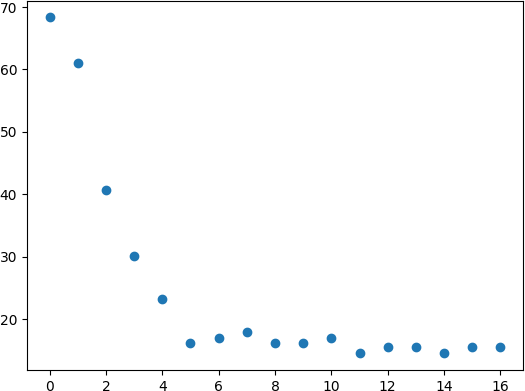
\includegraphics[width=0.7\textwidth]{fig/poids_sqrt}
      \caption{Racines carrées des intensités}
      \label{subfig:poids_sqrt}
    \end{subfigure}%
    \begin{subfigure}[t]{0.5\textwidth}
      \centering
      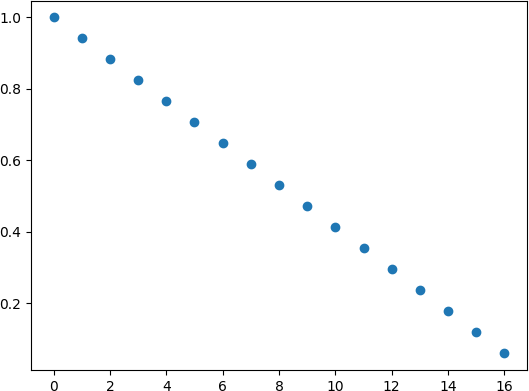
\includegraphics[width=0.7\textwidth]{fig/poids_triangle}
      \caption{Fonction triangulaire}
      \label{subfig:poids_triangle}
    \end{subfigure}%

  \end{figure}

\end{frame}

\begin{frame}{Ajustement : comparaison}
  \vspace{-0.4cm}
  \begin{columns}
    \begin{column}[c]{0.2\textwidth}
      \begin{figure}[ht]
        \centering
        Premier écho
        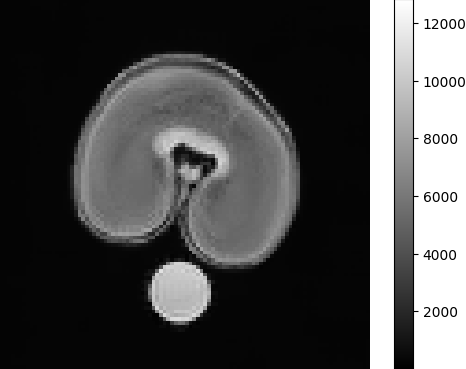
\includegraphics[width=0.9\linewidth]{fig/firstecho}
      \end{figure}
    \end{column}
    
    \begin{column}[c]{0.8\textwidth}
      \begin{figure}[ht]
    \begin{flushleft}
      Régression ($\sqrt{I})$
      \vspace{-0.1cm}
    \end{flushleft}
    \begin{subfigure}[t]{0.5\textwidth}
      \centering
      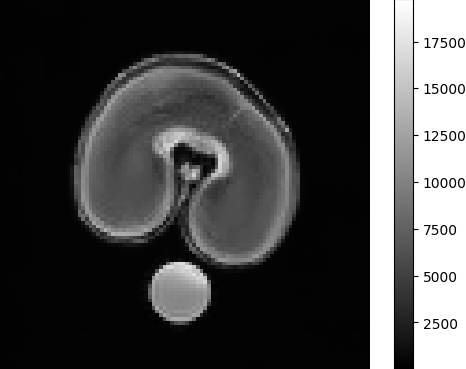
\includegraphics[width=0.5\textwidth]{fig/linear_regression_old}
    \end{subfigure}%
    \begin{subfigure}[t]{0.5\textwidth}
      \centering
      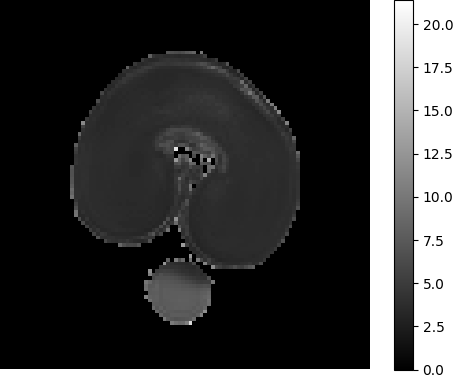
\includegraphics[width=0.5\textwidth]{fig/linear_regression_old_t2}
    \end{subfigure}%
    \begin{flushleft}
      Régression (triangulaire)
      \vspace{-0.25cm}
    \end{flushleft}
    \begin{subfigure}[t]{0.5\textwidth}
      \centering
      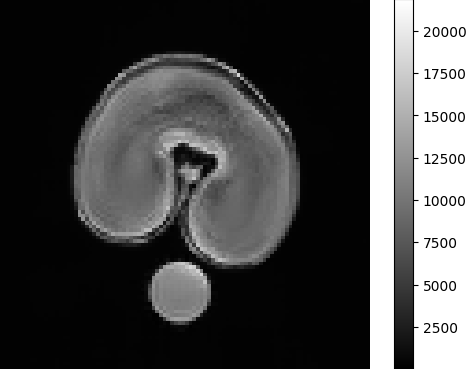
\includegraphics[width=0.5\textwidth]{fig/linear_regression_new}
    \end{subfigure}%
    \begin{subfigure}[t]{0.5\textwidth}
      \centering
      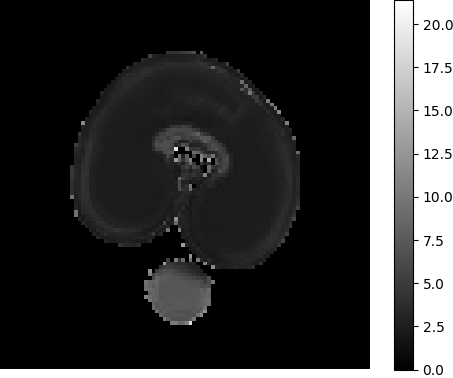
\includegraphics[width=0.5\textwidth]{fig/linear_regression_new_t2}
    \end{subfigure}
    \begin{flushleft}
      Moindres carrés
      \vspace{-0.25cm}
    \end{flushleft}
    \begin{subfigure}[t]{0.5\textwidth}
      \centering
      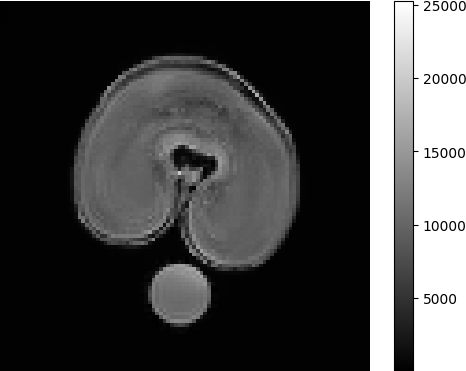
\includegraphics[width=0.5\textwidth]{fig/nnls}
    \end{subfigure}%
    \begin{subfigure}[t]{0.5\textwidth}
      \centering
      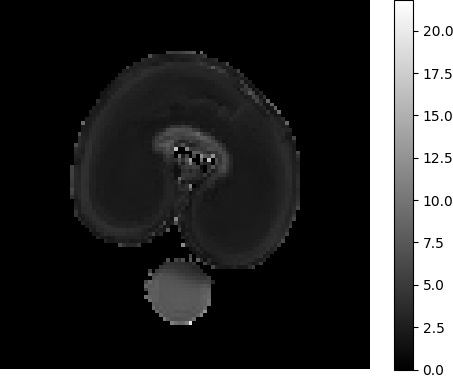
\includegraphics[width=0.5\textwidth]{fig/nnls_t2}
    \end{subfigure}%
      \end{figure}

    \end{column}
  \end{columns}
  


\end{frame}


\begin{frame}{Ajustement : évaluation quantitative}

  Erreurs résiduelles moyennes et temps de calcul:
  \vspace{-0.4cm}

  
  \begin{table}[]
    \begin{adjustbox}{max width=1\textwidth}
      \begin{tabular}{lllll}
        \hline
        & Par morceaux & \begin{tabular}[c]{@{}l@{}}Régression\\ ($\sqrt{I}$)\end{tabular} & \begin{tabular}[c]{@{}l@{}}Régression\\ (triangulaire)\end{tabular} & Moindres carrés \\ \hline
        Résidus (\%) & 1.09         & 1.21                                                            & 0.986                                                               & \textbf{0.941 }          \\
        t (s)   & 171          & \textbf{34}                                                              & \textbf{35}                                                                  & 261             \\ \hline
      \end{tabular}
  \end{adjustbox}
\end{table}

\vspace{0.2cm}

\textbf{Régression linéaire} : bonne approximation, temps de calcul court

\textbf{Moindres carrés} : plus précis, temps de calcul long


\end{frame}







\begin{frame}{Normalisation d'images de spectrométrie de masse}
  \cite{Deininger_2011}
\end{frame}




\appendix
\setbeamertemplate{headline}{%
  % \nointerlineskip
  % \begin{beamercolorbox}[wd=\paperwidth,leftskip=0.5cm,ht=0pt,dp=0pt]{block title}%
  %   \usebeamerfont{page number in head/foot}{\insertsection}
  % \end{beamercolorbox}%
  % \if@useTitleProgressBar
  % \nointerlineskip
  % % \vspace{-0.7cm}
  % \begin{beamercolorbox}[wd=\paperwidth,ht=0pt,dp=5pt]{section}
  %   \progressbar@titleprogressbar
  % \end{beamercolorbox}
  % \fi
  % \nointerlineskip
}

% \setbeamertemplate{frametitle}{%
%   \begin{beamercolorbox}[wd=\paperwidth,leftskip=0.7cm,rightskip=0.3cm,ht=0pt,dp=0pt]{frametitle}
%     \usebeamerfont{frametitle}\MakeLowercase{\protect\insertframetitle}
%   \end{beamercolorbox}
% }

\begin{frame}[allowframebreaks]
  \frametitle{Références}
  \setbeamertemplate{bibliography item}{$\bullet$}
  \bibliographystyle{apalike}
  \scriptsize{
    \bibliography{main}
  }
\end{frame}



\end{document}
